% 原始 SWE-agent 概览图：只替换实际存在的自然语言接口标签，ACI/UI 和图标原样保留。
\begingroup
\definecolor{ch13SweAgent}{RGB}{228,238,253}
\definecolor{ch13SweComputer}{RGB}{248,222,209}
\definecolor{ch13SweViewer}{RGB}{168,217,251}
\definecolor{ch13SweEditor}{RGB}{209,189,250}
\definecolor{ch13SweSearch}{RGB}{251,232,156}
\definecolor{ch13SweHuman}{RGB}{233,243,235}
\newlength{\chThirteenSweUnit}
\setlength{\chThirteenSweUnit}{\dimexpr\linewidth/2168\relax}
\begin{tikzpicture}[x=\chThirteenSweUnit,y=-\chThirteenSweUnit]
  \node[anchor=north west,inner sep=0pt] at (0,0) {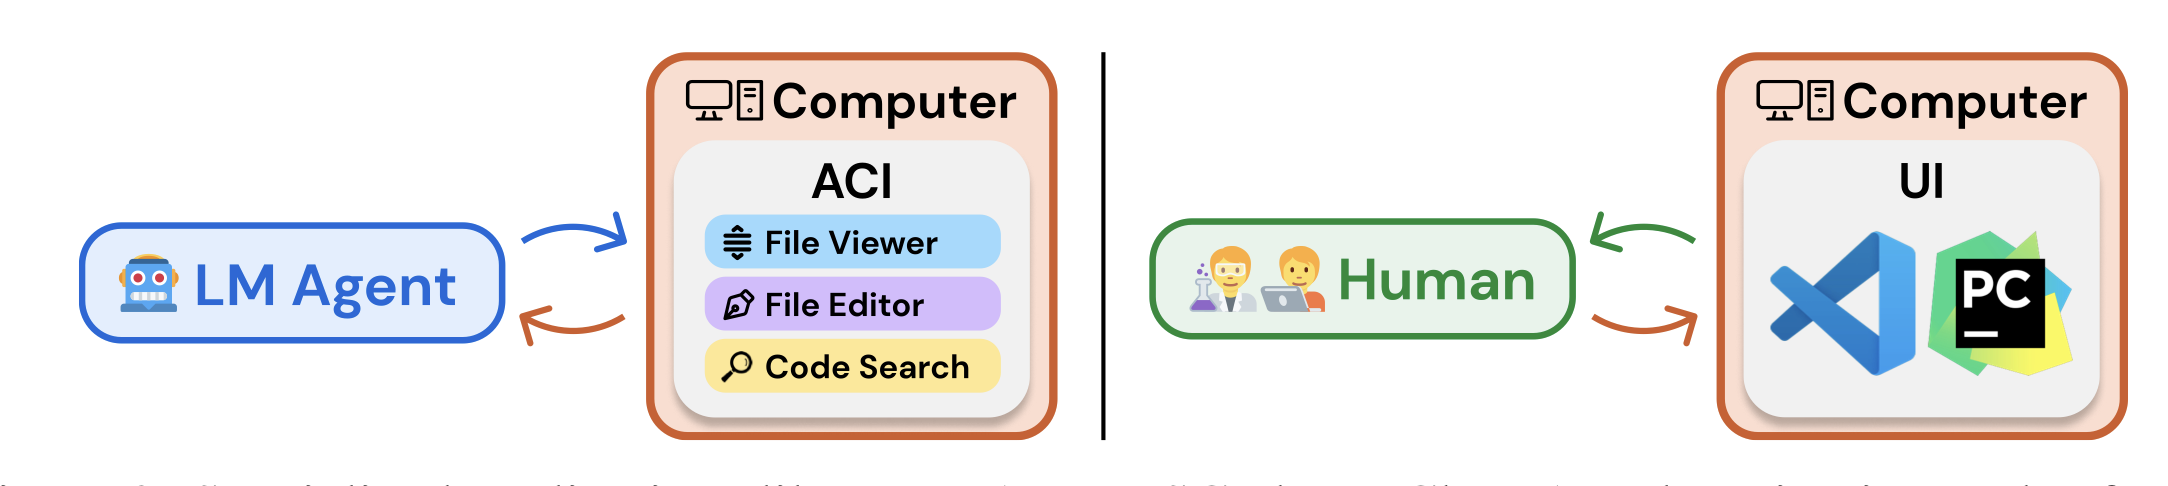
\includegraphics[width=\linewidth]{figures/swe.png}};
  \fill[ch13SweAgent] (185,252) rectangle (492,317);
  \node[text=blue!68!cyan!78!black,font=\fontsize{8.5}{10}\selectfont\bfseries] at (339,286) {语言模型智能体};
  \fill[ch13SweComputer] (771,76) rectangle (1035,126);
  \node[font=\fontsize{11}{13}\selectfont\bfseries] at (901,103) {计算机};
  \fill[ch13SweComputer] (1839,76) rectangle (2104,126);
  \node[font=\fontsize{11}{13}\selectfont\bfseries] at (1971,103) {计算机};
  \fill[ch13SweViewer] (758,225) rectangle (989,260);
  \node[font=\fontsize{8.8}{10}\selectfont\bfseries] at (873,244) {文件查看器};
  \fill[ch13SweEditor] (758,287) rectangle (989,324);
  \node[font=\fontsize{8.8}{10}\selectfont\bfseries] at (873,306) {文件编辑器};
  \fill[ch13SweSearch] (758,348) rectangle (989,387);
  \node[font=\fontsize{8.8}{10}\selectfont\bfseries] at (873,368) {代码搜索};
  \fill[ch13SweHuman] (1332,252) rectangle (1544,310);
  \node[text=green!45!black,font=\fontsize{12}{14}\selectfont\bfseries] at (1438,282) {人类};
\end{tikzpicture}
\endgroup
